\begin{frame}
    \frametitle{Preparation: feature extraction}
    Apply "compute descriptors" tool from \alert{University of Surrey} with the following parameters:
    \begin{center}
        \textbf{-hesaff -sift -noangle}
    \end{center}
    \textbf{hesaff}: Scale and Affine invariant interest point detector\\
    \textbf{sift}: use Scale Invariant Feature Transform (SIFT) descriptor\\
    \textbf{noangle}: no angle estimation
\end{frame}

\begin{frame}
    \frametitle{Preparation: feature extraction}
    \begin{center}
    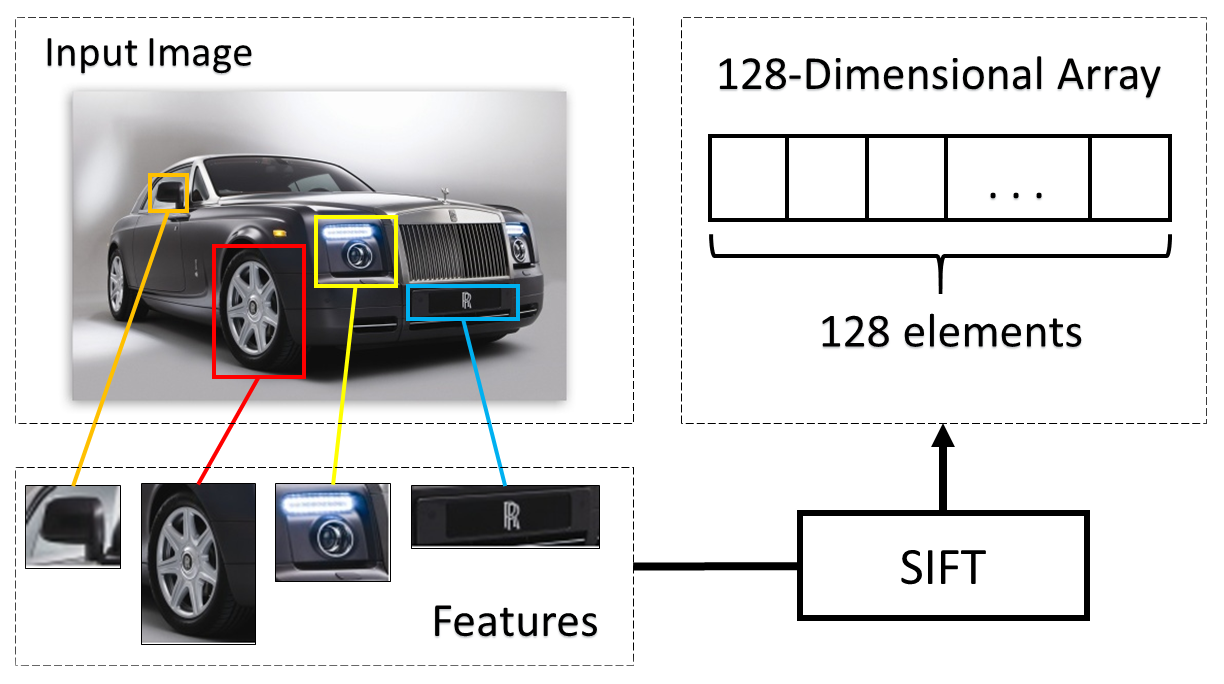
\includegraphics[width=\textwidth]{images/feature_extraction2.png}
    \end{center}
\end{frame}

\begin{frame}
    \frametitle{Preparation: codebook building}
    Use \textbf{approximate k-Means} to cluster all features to \textbf{1M} clusters
    \begin{itemize}
        \item Use \alert{FASTANN} and \alert{FASTCLUSTER} libraries \footcite{Muja M. and Lowe D., Fast approximate nearest neighbours with automatic algorithm configuration, Proceedings VISAPP 2009} \footcite{Philbin J. Chum O. Isard M. Sivic J. and Zisserman A., Object retrieval with large vocabularies and fast spatial matching, Proceedings CVPR 2007}
        \item Run with \textbf{50} iterations
    \end{itemize}
    Each image is presented by a \textbf{1M-dimensional} vector
\end{frame}

\begin{frame}
    \frametitle{Preparation: codebook building}
    \begin{figure}
        \centering
        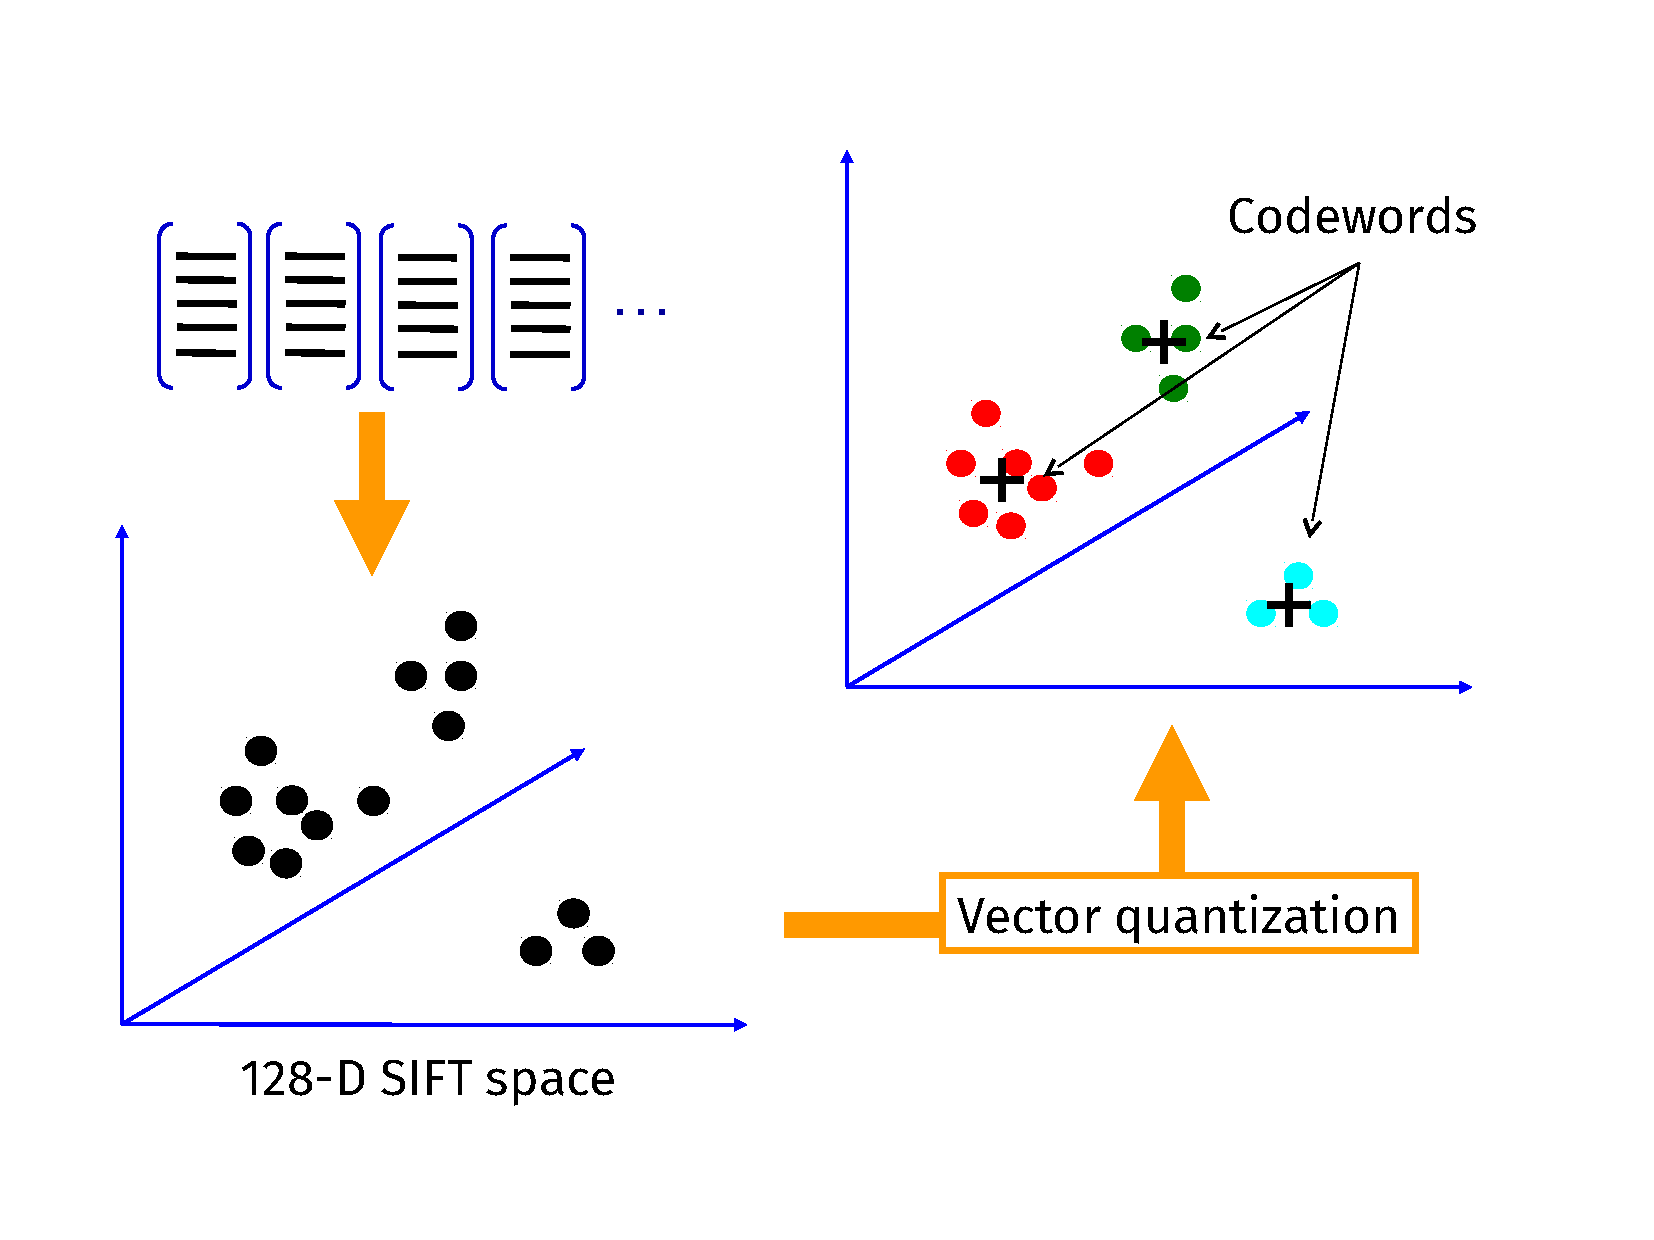
\includegraphics[width=3.3in]{images/cluster.pdf}
        \caption{Clustering \footcite{Slide credit: Josef Sivic}}
    \end{figure}
\end{frame}

\begin{frame}
    \frametitle{Preparation: quantization}
    \textbf{Soft assignment:} Each \textbf{128-dimensional} feature vector is reduced to \textbf{3-dimensional} by looking for its \textbf{3 nearest visual words}\\
    Each of the \textbf{nearest visual words} is assigned with \alert{weight}:
    \begin{equation*}
        weight = exp(-\frac{d^2}{2\delta^2})
    \end{equation*}
\hspace{4ex} $d = $ distance from feature vector to cluster centroid

\hspace{4ex} $\delta^2 = 6250$\\

    All weights are added to their corresponding visual word in the \textbf{1M-dimensional} representation of the image
\end{frame}


\begin{frame}
    \frametitle{Preparation: quantization}
    \begin{center}
    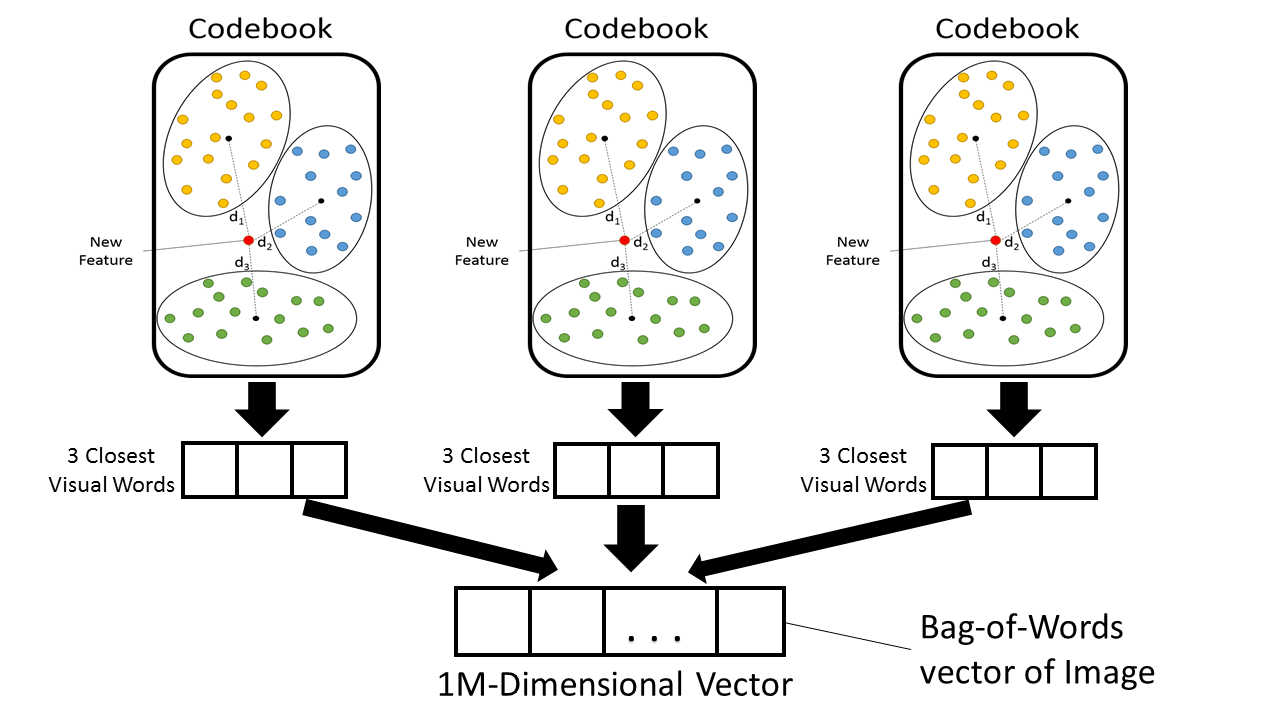
\includegraphics[width=\textwidth]{images/quantization.png}
    \end{center}
\end{frame}

\begin{frame}
    \frametitle{Query: tf-idf weighting}
    Similar with text retrieval
    \begin{itemize}
        \item \textbf{raw term frequency:} $raw\;tf_{i,j} =$ weight of visual word i in image j
        \item \textbf{document frequency:} $df_i =$ \# of images that visual word i appears
        \item \textbf{raw inverse document frequency:} $raw\;idf_i = |D|/df_i$
    \end{itemize}   
\end{frame}

\begin{frame}
    \frametitle{Query: tf-idf weighting}
    Observation
    \begin{itemize}
        \item The \textbf{more time} a visual word occurs, the \textbf{less important} it is
        \item A visual word is \textbf{more discriminate} if it occurs in \textbf{fewer} images
    \end{itemize}
    Hence, it is necessary to \textbf{normalize} the \textbf{values of TF-IDF}
    
    \hspace{4ex}$tf_{i,j} =  \frac{raw\;tf_{i,j}}{\sum\limits_{k}raw\;tf_{k,j}}$ (for all visual words k in image j)
    
    \hspace{4ex}$idf_{i} = \log{\frac{|D|}{|\{j:t_{i}\in d_{j}\}|}}$
\end{frame}

\begin{frame}
    \frametitle{Query: tf-idf weighting}
    Weight of visual word i in image j is therefore: $tfidf_{i,j} = tf_{i,j}\times idf_{i}$\\\\
    The tf-idf weight is used to \textbf{compute similarity} between an image $d_{i}$ and a query $q$
    \begin{equation*}
        s_{d_{i},q} = \vec{{tfidf}_{i}} \cdot \vec{{tfidf}_{q}} = \sum\limits_{j = 1}^{\left|T\right|} {tfidf}_{i, j} \times {tfidf}_{q, j}
    \end{equation*}
    By \textbf{sorting} list of images based on their \textbf{similarity score} with a query, we achieve the \textbf{raw ranked list} which is used for the \textbf{Query Expansion} step
\end{frame}

\begin{frame}
    \frametitle{Query: Query expansion}
    Apply \textbf{geometric verification} between the query image \textbf{Q} and each top-ranked image \textbf{A}:
    \begin{enumerate}
        \item $(x,y)$ is a \textbf{matched pair} of features if $x \in Q$, $y \in A$, x and y are assigned to the same visual word
        \item Randomly choose 4 pairs of features to build the \textbf{homography matrix}. A matched pair $(x,y)$ is called \textbf{inliner} if apply the computed homography matrix on feature x produces feature y. Repeat 100 times to find the matrix that produces the \textbf{largest} number of inliners. These inliers are the \textbf{verified} visual words
        \item \textbf{TF-IDF weight} of the \textbf{verified} visual words are added to query
    \end{enumerate}
    Run this process for all top-ranked images. The added TF-IDF weight are averaged before running the query again
\end{frame}

